% --- Statistical rigor ---
\begin{frame}[allowframebreaks]{An Eval Score Is an Estimate, Not a Measurement}
  \begin{itemize}\footnotesize\itemsep0.3em
    \item[\textcolor{red}{$\blacktriangleright$}] Almost every eval table in the literature reports point estimates with no uncertainty, and readers duly compare 71.2 against 70.8. The right frame is that your questions were \textbf{drawn from an unseen super-population} of questions you could have asked; the score is a sample mean.
    \item[\textcolor{red}{$\blacktriangleright$}] With $n$ questions and per-question scores $s_1,\dots,s_n$, the Central Limit Theorem gives
      \[
        \mathrm{SE}_{\mathrm{CLT}} = \sqrt{\frac{\widehat{\mathrm{Var}}(s)}{n}}
          = \sqrt{\frac{1}{n} \cdot \frac{1}{n-1}\sum_{i=1}^{n}\left(s_i - \bar{s}\right)^2},
        \qquad
        \mathrm{CI}_{95\%} = \bar{s} \pm 1.96\,\mathrm{SE}_{\mathrm{CLT}}.
      \]
    \item[\textcolor{red}{$\blacktriangleright$}] For a pass/fail eval each $s_i$ is Bernoulli, so this simplifies to $\mathrm{SE} = \sqrt{\bar{s}(1-\bar{s})/n}$.
    \item[\textcolor{red}{$\blacktriangleright$}] \textbf{Work an example.} MT-Bench's 80 questions, scored pass/fail near $\bar{s} = 0.75$, give $\mathrm{SE} = \sqrt{0.75 \times 0.25/80} \approx 0.048$ --- a 95\% interval nearly \textbf{19 points wide}. A 3-point ``improvement'' on 80 questions is indistinguishable from noise.
    \item[\textcolor{red}{$\blacktriangleright$}] Precision improves as $1/\sqrt{n}$: halving the interval costs $4\times$ the questions. This is why benchmark size is a design decision, not an afterthought.
    \item[\textcolor{red}{$\blacktriangleright$}] \textbf{Minimum standard:} report $n$ and a standard error next to every number. Everything else in this section refines this estimate; nothing replaces it.
  \end{itemize}
  \vspace{0.1em}
  {\scriptsize Following Miller, ``Adding Error Bars to Evals: A Statistical Approach to Language Model Evaluations,'' Anthropic, \href{https://arxiv.org/abs/2411.00640v1}{arXiv:2411.00640v1}, Eqs.~1--3.}
\end{frame}

\begin{frame}[allowframebreaks]{Clustered Questions Break the Independence Assumption}
  \begin{itemize}\footnotesize\itemsep0.32em
    \item[\textcolor{red}{$\blacktriangleright$}] The CLT formula assumes questions are independent draws. Eval sets routinely violate this:
      \begin{itemize}\itemsep0.12em
        \item Reading-comprehension items sharing one passage --- miss the passage, miss all its questions.
        \item MMLU's 57 subjects, where items within a subject share vocabulary and source material.
        \item Multi-turn conversations scored turn by turn.
        \item Several paraphrases of the same underlying question.
      \end{itemize}
    \item[\textcolor{red}{$\blacktriangleright$}] Within a cluster, scores are \textbf{positively correlated}, so the effective sample size is closer to the number of \textit{clusters} than the number of questions. Ignoring this makes your intervals too narrow and your differences look significant when they are not.
    \item[\textcolor{red}{$\blacktriangleright$}] The correction adds the within-cluster cross-products back in:
      \[
        \mathrm{SE}_{\text{clustered}} = \left(\mathrm{SE}_{\mathrm{CLT}}^{2}
          + \frac{1}{n^{2}}\sum_{c}\sum_{i}\sum_{j \neq i}
            \left(s_{i,c} - \bar{s}\right)\left(s_{j,c} - \bar{s}\right)\right)^{1/2},
      \]
      where $s_{i,c}$ is the score on question $i$ in cluster $c$.
    \item[\textcolor{red}{$\blacktriangleright$}] If you bootstrap instead of using a formula, \textbf{resample clusters, not questions}. Resampling questions inside clusters reproduces exactly the bias you are trying to remove.
    \item[\textcolor{red}{$\blacktriangleright$}] \textbf{Design implication:} adding a fifth question about a passage you already use buys far less precision than adding a new passage. Breadth beats depth for statistical power.
  \end{itemize}
\end{frame}

\begin{frame}[allowframebreaks]{Comparing Two Models: Pair the Questions}
  \begin{itemize}\footnotesize\itemsep0.3em
    \item[\textcolor{red}{$\blacktriangleright$}] The question is almost never ``how good is model A'' but ``is A better than B''. Both were run on \textbf{the same questions}, so the comparison should be made \textbf{question by question}, not by subtracting two independent means.
    \item[\textcolor{red}{$\blacktriangleright$}] Define $s_{A-B,i} = s_{A,i} - s_{B,i}$ and analyse that single series. Its standard error is
      \[
        \mathrm{SE}_{A-B}^{\text{paired}}
          = \sqrt{\mathrm{SE}_A^2 + \mathrm{SE}_B^2 - 2\,\mathrm{SE}_A\,\mathrm{SE}_B\,\mathrm{Corr}(s_A, s_B)},
      \]
      whereas treating the runs as independent drops the covariance term entirely and gives $\sqrt{\mathrm{SE}_A^2 + \mathrm{SE}_B^2}$.
    \item[\textcolor{red}{$\blacktriangleright$}] That third term is large in practice: two models find \textit{the same} questions hard, so $\mathrm{Corr}$ is high. At $\mathrm{Corr} = 0.5$ pairing removes about \textbf{a third of the variance} for free --- the same precision from two thirds of the data.
    \item[\textcolor{red}{$\blacktriangleright$}] \textbf{Variance reduction, second lever.} Each score has a question component and a sampling component. Drawing $K$ answers per question and averaging shrinks the conditional variance to $\sigma_i^2/K$, with diminishing returns once it is small relative to the between-question variance $\mathrm{Var}(x)$.
    \item[\textcolor{red}{$\blacktriangleright$}] \textbf{Best case:} for single-token multiple choice, score the \textbf{next-token probability} instead of a sampled letter. The sampling noise becomes exactly zero, and $\mathrm{Var}(\hat{\mu}) = \mathrm{Var}(p)/n$ --- free precision, no extra inference.
    \item[\textcolor{red}{$\blacktriangleright$}] For binary paired outcomes the classical test is \textbf{McNemar's}: only the discordant pairs (one model right, the other wrong) carry information, so an eval where both models agree everywhere has no power however large it is.
  \end{itemize}
  \vspace{0.1em}
  {\scriptsize Miller, \href{https://arxiv.org/abs/2411.00640v1}{arXiv:2411.00640v1}, Eqs.~5--7.}
\end{frame}

\begin{frame}{Power Analysis: Is This Eval Capable of Answering the Question?}
  \begin{itemize}\footnotesize\itemsep0.3em
    \item[\textcolor{red}{$\blacktriangleright$}] Run this \textbf{before} the experiment, not after. Given a smallest difference $\delta$ worth detecting, significance level $\alpha$, and power $1-\beta$, the required number of questions is
      \[
        n = \frac{\left(z_{\alpha/2} + z_{\beta}\right)^{2}
              \left(\omega^{2} + \sigma_A^{2}/K_A + \sigma_B^{2}/K_B\right)}{\delta^{2}},
        \qquad
        \omega^{2} = \mathrm{Var}(x_A) + \mathrm{Var}(x_B) - 2\,\mathrm{Cov}(x_A, x_B),
      \]
      where $K_A, K_B$ are the answers sampled per question and $\omega^2$ is the paired between-question variance.
    \item[\textcolor{red}{$\blacktriangleright$}] Inverted, it tells you the \textbf{minimum detectable effect} of the eval you already have:
      $\delta = (z_{\alpha/2} + z_{\beta})\sqrt{(\omega^2 + \sigma_A^2/K_A + \sigma_B^2/K_B)/n}$.
      Compute this once for each of your suites and write it on the dashboard. It converts ``the number went up'' into ``the number went up by more than this eval can resolve''.
    \item[\textcolor{red}{$\blacktriangleright$}] Two structural facts fall out. First, $\delta$ shrinks only as $1/\sqrt{n}$, so \textbf{detecting a 1-point difference needs roughly 100$\times$ the data of a 10-point difference}. Second, since $\omega^2$ contains the covariance term, \textbf{an eval that is too small to rank models absolutely may still be plenty for a paired A/B test}.
    \item[\textcolor{red}{$\blacktriangleright$}] \textbf{The honest outcome of a power analysis is often ``this eval cannot answer this question.''} Say so rather than reporting the point estimate and letting the reader assume otherwise.
  \end{itemize}
  \vspace{0.1em}
  {\scriptsize Miller, \href{https://arxiv.org/abs/2411.00640v1}{arXiv:2411.00640v1}, Eq.~9.}
\end{frame}

\begin{frame}{Small Samples, and Many Comparisons}
  \begin{columns}[T,onlytextwidth]
    \column{0.5\textwidth}
      {\scriptsize \textbf{When$n$ is small or the score is near 0 or 1}}
      \begin{itemize}\footnotesize\itemsep0.05em
        \item[\textcolor{red}{$\blacktriangleright$}] The normal (Wald) interval $\hat{\theta} \pm z\sqrt{\hat{\theta}(1-\hat{\theta})/n}$ \textbf{collapses to zero width} at $\hat{\theta} \in \{0,1\}$ and can run outside $[0,1]$. Its coverage is erratic even at large $n$.
        \item[\textcolor{red}{$\blacktriangleright$}] Use the \textbf{Wilson score interval}, which inverts the score test and stays inside $[0,1]$:
          \[
            \frac{\hat{\theta} + \frac{z^2}{2n}}{1 + \frac{z^2}{n}}
            \;\pm\;
            \frac{z}{1 + \frac{z^2}{n}}
            \sqrt{\frac{\hat{\theta}(1-\hat{\theta})}{n} + \frac{z^2}{4n^2}}.
          \]
        \item[\textcolor{red}{$\blacktriangleright$}] Below a few hundred datapoints, do not use CLT intervals at all. Bowyer et al.\ show that \textbf{bootstrap intervals also under-cover badly} at small $n$, and recommend \textbf{Wilson} or \textbf{Bayesian} intervals from the Beta posterior
          $\mathrm{Beta}\!\left(1 + \sum_i y_i,\ 1 + \sum_i (1 - y_i)\right)$.
        \item[\textcolor{red}{$\blacktriangleright$}] Bootstrap remains the right tool for \textbf{large $n$} and \textbf{non-linear metrics} (F1, nDCG, Bradley--Terry coefficients), where no closed form exists.
      \end{itemize}
    \column{0.48\textwidth}
      {\scriptsize \textbf{Whenyou run many tests}}
      \begin{itemize}\footnotesize\itemsep0.05em
        \item[\textcolor{red}{$\blacktriangleright$}] Comparing $M$ models on $K$ benchmarks is $MK$ --- or $\binom{M}{2}K$ --- simultaneous tests. At $\alpha = 0.05$, roughly one in twenty ``wins'' is noise, and a leaderboard has hundreds of cells.
        \item[\textcolor{red}{$\blacktriangleright$}] Control the family-wise error rate with \textbf{Holm's step-down procedure} --- strictly more powerful than Bonferroni at no extra cost or assumption --- or control the false discovery rate with \textbf{Benjamini--Hochberg} when you want discovery power rather than strict protection.
        \item[\textcolor{red}{$\blacktriangleright$}] For the specific shape ``many models across many datasets'', the standard recipe is \textbf{Wilcoxon signed-ranks} for two models and \textbf{Friedman with a Nemenyi post-hoc} for several.
        \item[\textcolor{red}{$\blacktriangleright$}] This is exactly why the Chatbot Arena leaderboard applies a multiplicity correction to its Bradley--Terry intervals.
      \end{itemize}
  \end{columns}
  {\scriptsize Brown, Cai \& DasGupta, ``Interval Estimation for a Binomial Proportion,'' \textit{Statistical Science} 16(2), 2001; Bowyer, Aitchison \& Ivanova, ICML 2025, \href{https://arxiv.org/abs/2503.01747v3}{arXiv:2503.01747v3}; Dem\v{s}ar, \textit{JMLR} 7:1--30, 2006.}
\end{frame}

\begin{frame}{The Variance You Did Not Control For}
  \begin{columns}[T,onlytextwidth]
    \column{0.5\textwidth}
      \begin{itemize}\footnotesize\itemsep0.05em
        \item[\textcolor{red}{$\blacktriangleright$}] Sampling error over questions is only one source. HELM measured another directly: re-run each scenario with \textbf{three different random sets of in-context examples} and take the range of accuracy across seeds.
        \item[\textcolor{red}{$\blacktriangleright$}] Result: mostly reassuring but not uniformly so. The median range across scenarios is \textbf{below 0.03 for 24 of 28 models}; the exceptions were YaLM~(100B) and three GPT-3 variants. Some \textit{scenarios} are high-variance for everyone --- NaturalQuestions (open-book) prominently.
        \item[\textcolor{red}{$\blacktriangleright$}] Stack the sources: question sampling ($\pm$ a few points on a small suite), few-shot seed ($\approx 3$ points), prompt format (median 7.5 points, up to 76), decoding temperature, judge version, and harness version.
        \item[\textcolor{red}{$\blacktriangleright$}] \textbf{Any of these can exceed the difference you are reporting.} That is the practical reason so many published improvements do not replicate.
      \end{itemize}
    \column{0.48\textwidth}
      \centering
      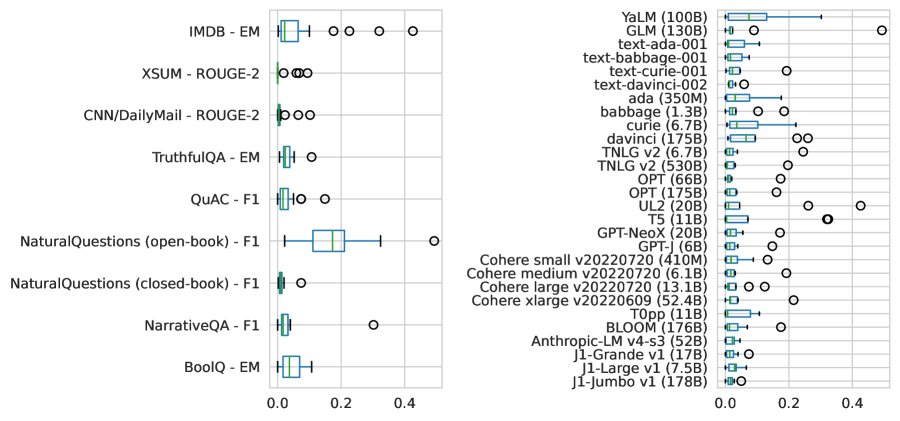
\includegraphics[width=\linewidth,height=0.3\textheight,keepaspectratio]{images/llm-evaluation/helm_fig31_variance_across_seeds.png}\\[0.1em]
      {\scriptsize ``Variance across seeds. For a subset of models and scenarios, we evaluate each scenario with three different random sets of in-context examples. We compute the range of the accuracy metric (maximum minus minimum value over the three random seeds).'' Liang et al., \href{https://arxiv.org/abs/2211.09110v2}{arXiv:2211.09110v2}, Figure 31.}
      \begin{itemize}\footnotesize\itemsep0.05em
        \item[\textcolor{red}{$\blacktriangleright$}] \textbf{Reporting minimum:} $n$, standard error, seeds, prompt format, decoding parameters, harness and judge versions, and the contamination check you ran. Anything less is not reproducible.
      \end{itemize}
  \end{columns}
\end{frame}
